\begin{frame}{Motivation}


 \begin{itemize}
  \item Web Search is a quest for Structure \medskip
  \item The open web is huge, \textbf{1.8 billion} indexed web pages\footnote{As of 31st March 2014}, but unstructured  \medskip
  \item The knowledge is scattered around in pieces \medskip
  \item A user needs to carve the structure out of the web  \medskip

 
 \end{itemize}

\end{frame}

\begin{frame}
\begin{exampleblock}{}
  {\large ``Words that you use when you are doing the search, well they aren't \emph{just words}, they refer to \textbf{real} things
in the world``}
  \vskip5mm
  \hspace*\fill{\small--- Jack Menzel, Product Management Director, Google Knowledge Graph
}
\end{exampleblock}
\end{frame}

\begin{frame}{Structuring the web}
 \begin{itemize}
   \item Structuring the web : A web page is more than just a bundle of strings \medskip
  \item Learn what the text is all about \medskip
  \item Go beyond web of strings to the web of entities \medskip
   \begin{center}``Albert Einstein'' \end{center}\medskip
  \item Beyond the tricks like finding pages having the \textbf{String} ``Albert Einstein'', \medskip
  pages which link to pages having the \textbf{String} ``Albert Einstein''
  
 \end{itemize}

\end{frame}


\begin{frame}
 \frametitle{Words are not just words}
\begin{textblock*}{100pt}[.50,.5](190pt,170pt)
\begin{figure}[h]
 \centering
 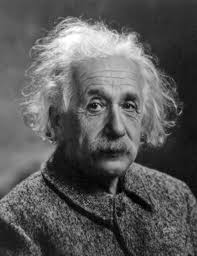
\includegraphics[bb=0 0 197 256,scale=0.5]{./einstein.jpg}
  \caption{Albert Einstein}
 % einstein.jpg: 197x256 pixel, 72dpi, 6.95x9.03 cm, bb=0 0 197 256
\end{figure}
\end{textblock*}
\end{frame}
\begin{frame}
 \frametitle{Words are not just words}
\begin{textblock*}{100pt}[.50,.5](190pt,170pt)
\begin{figure}[h]
 \centering
 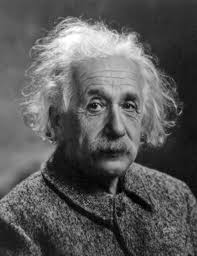
\includegraphics[bb=0 0 197 256,scale=0.5]{./einstein.jpg}
  \caption{Albert Einstein}
 % einstein.jpg: 197x256 pixel, 72dpi, 6.95x9.03 cm, bb=0 0 197 256
\end{figure}
\end{textblock*}
\begin{textblock*}{80pt}[.50,.5](60pt,70pt)
\begin{figure}[h]
 \centering
 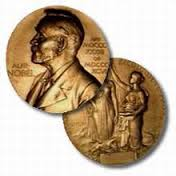
\includegraphics[bb=0 0 197 256,scale=0.5]{./nobel.jpg}
 % einstein.jpg: 197x256 pixel, 72dpi, 6.95x9.03 cm, bb=0 0 197 256
\end{figure}
\end{textblock*}

\end{frame}
\begin{frame}
 \frametitle{Words are not just words}
\begin{textblock*}{100pt}[.50,.5](190pt,170pt)
\begin{figure}[h]
 \centering
 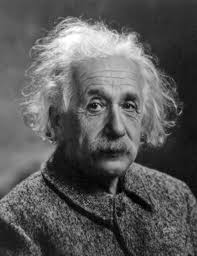
\includegraphics[bb=0 0 197 256,scale=0.5]{./einstein.jpg}
  \caption{Albert Einstein}
 % einstein.jpg: 197x256 pixel, 72dpi, 6.95x9.03 cm, bb=0 0 197 256
\end{figure}
\end{textblock*}
\begin{textblock*}{80pt}[.50,.5](60pt,70pt)
\begin{figure}[h]
 \centering
 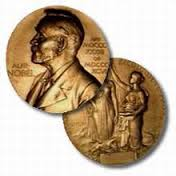
\includegraphics[bb=0 0 197 256,scale=0.5]{./nobel.jpg}
 % einstein.jpg: 197x256 pixel, 72dpi, 6.95x9.03 cm, bb=0 0 197 256
\end{figure}
\end{textblock*}

\begin{textblock*}{80pt}[.50,.5](60pt,170pt)
\begin{figure}[h]
 \centering
 
\includegraphics[bb=0 0 197 256,scale=0.5]{./zurich.jpg}
 % einstein.jpg: 197x256 pixel, 72dpi, 6.95x9.03 cm, bb=0 0 197 256
\end{figure}
\end{textblock*}

\end{frame}
\begin{frame}
 \frametitle{Words are not just words}
\begin{textblock*}{100pt}[.50,.5](190pt,170pt)
\begin{figure}[h]
 \centering
 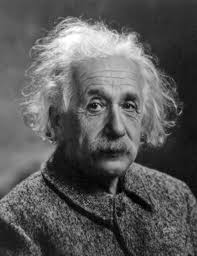
\includegraphics[bb=0 0 197 256,scale=0.5]{./einstein.jpg}
 % einstein.jpg: 197x256 pixel, 72dpi, 6.95x9.03 cm, bb=0 0 197 256
 \caption{Albert Einstein}
\end{figure}
\end{textblock*}
\begin{textblock*}{80pt}[.50,.5](60pt,70pt)
\begin{figure}[h]
 \centering
 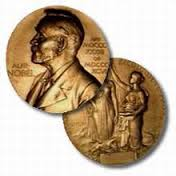
\includegraphics[bb=0 0 197 256,scale=0.5]{./nobel.jpg}
 % einstein.jpg: 197x256 pixel, 72dpi, 6.95x9.03 cm, bb=0 0 197 256
\end{figure}
\end{textblock*}

\begin{textblock*}{80pt}[.50,.5](60pt,170pt)
\begin{figure}[h]
 \centering
 
\includegraphics[bb=0 0 197 256,scale=0.5]{./zurich.jpg}
 % einstein.jpg: 197x256 pixel, 72dpi, 6.95x9.03 cm, bb=0 0 197 256
\end{figure}
\end{textblock*}


\begin{textblock*}{120pt}[.50,.5](310pt,70pt)
\begin{itemize} 
\item \textbf{Born :} 1879, Germany
\item \textbf{Died :} 1955, US
 \end{itemize}
\end{textblock*}
\end{frame}
\begin{frame}
 \frametitle{Words are not just words}
\begin{textblock*}{100pt}[.50,.5](190pt,170pt)
\begin{figure}[h]
 \centering
 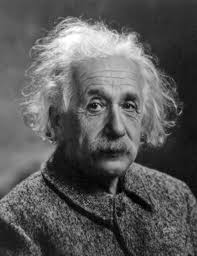
\includegraphics[bb=0 0 197 256,scale=0.5]{./einstein.jpg}
 % einstein.jpg: 197x256 pixel, 72dpi, 6.95x9.03 cm, bb=0 0 197 256
 \caption{Albert Einstein}
\end{figure}
\end{textblock*}
\begin{textblock*}{80pt}[.50,.5](60pt,70pt)
\begin{figure}[h]
 \centering
 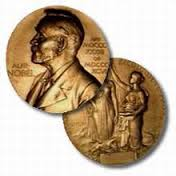
\includegraphics[bb=0 0 197 256,scale=0.5]{./nobel.jpg}
 % einstein.jpg: 197x256 pixel, 72dpi, 6.95x9.03 cm, bb=0 0 197 256
\end{figure}
\end{textblock*}

\begin{textblock*}{80pt}[.50,.5](60pt,170pt)
\begin{figure}[h]
 \centering
 
\includegraphics[bb=0 0 197 256,scale=0.5]{./zurich.jpg}
 % einstein.jpg: 197x256 pixel, 72dpi, 6.95x9.03 cm, bb=0 0 197 256
\end{figure}
\end{textblock*}


\begin{textblock*}{120pt}[.50,.5](310pt,70pt)
\begin{itemize} 
\item \textbf{Born :} 1879, Germany
\item \textbf{Died :} 1955, US
 \end{itemize}

\end{textblock*}

\begin{textblock*}{120pt}[.50,.5](310pt,170pt)
''Entities'' \emph{like} Albert Einstein
\begin{itemize} 
\item \textbf{Born :} Issac Newton
\item \textbf{Died :} Stephen Hawking
 \end{itemize}
\end{textblock*}

\end{frame}

